\documentclass[useAMS,usenatbib]{mn2e}

\voffset=-0.8in

% Packages:
\usepackage{graphicx}
\usepackage{amsmath}
\usepackage{xspace}
\usepackage{dsfont}
\usepackage[utf8]{inputenc}
\usepackage{caption}
\usepackage{subcaption} % subfigures
\usepackage{float}

\title[]
{Lensing}
    
\author[Brewer, Huijser and Lewis]{%
  Brendon~J.~Brewer$^{1}$\thanks{bj.brewer@auckland.ac.nz},
  David Huijser$^{1}$,
  Geraint F. Lewis$^2$
  \medskip\\
  $^1$Department of Statistics, The University of Auckland, Private Bag 92019, Auckland 1142, New Zealand\\
  $^2$Sydney Institute for Astronomy, School of Physics, A28,
  The University of Sydney, NSW 2006, Australia}

%%%%%%%%%%%%%%%%%%%%%%%%%%%%%%%%%%%%%%%%%%%%%%%%%%%%%%%%%%%%%%%%%%%%%%%%%%%%%%

\begin{document}
             
\date{To be submitted to MNRAS}
             
\maketitle

\label{firstpage}

\begin{abstract}

\end{abstract}


\begin{keywords}
methods: data analysis --- methods: statistical
\end{keywords}

\section{Introduction}
Galaxy-galaxy lensing is a powerful astrophysical tool for studying
the distribution of matter, including dark matter, in galaxies
\citep{treu}. In recent years, several lens systems have been discovered which
are thought to contain at least one dark substructure
\citep{vegetti1, vegetti2, vegetti3}. In this paper we address the topic of
inferring the matter distribution in the lens galaxy from the lensed,
blurred image. These approaches may be categorized according to
Whether to use a simply parameterized (e.g. Sérsic)
or flexible (e.g. pixellated) model for the surface brightness profile of the source
\item Whether to use a simply parameterized (e.g. Singular Isothermal Ellipsoid)
or flexible model (e.g. pixellated) for the mass profile of the lens
\item How to compute the results (e.g. optimization methods, Markov Chain

Many different approaches have been proposed and applied to
this problem. The differences between the approaches can be broken down into
i) different assumptions about the prior information being used, and ii)
different computational methods used to compute the results.
Each approach involves tradeoffs between convenience and realism.
Simply parameterized models, such as Sérsic surface
brightness profiles for the source, and SIE models for the lens, are very
convenient. They only have a few adjustable parameters, and they capture
(to ``first order'') relevant prior information that we have about the
source and lens profiles. Of course, they are clearly simplifications,
and can produce misleading results if the actual profile is very different
from any member of the assumed family.

On the
other hand, pixellated models for the source \citep[e.g.][]{suyu} or the lens
\citep[e.g.][]{2014MNRAS.445.2181C} can in principle represent ``any''
source surface brightness profile or lens density profile. However, the prior
distribution over pixel values is often chosen to be a multivariate gaussian
for mathematical reasons, so
that the source can be analytically marginalized over
\citep{2003ApJ...590..673W}. Unfortunately, a multivariate gaussian prior
over pixel intensities can correspond to a very poor model of our prior
beliefs about the source. It assigns virtually zero prior probability
to the hypothesis that the source actually looks like a galaxy, and very high
prior probability to the hypothesis that the source looks like noise (or
blurred noise).

In a previous paper \citep{2011MNRAS.412.2521B} we argued that an ideal
modelling approach lies somewhere between simply-parameterised and
pixellated models. The source and the lens can be built up from a moderate
number of simply parameterised components. For the source, this allows
us to incorporate prior knowledge about the local correlations (the surface
brightness at any particular point is likely to be similar to that at a
nearby point) and the fact that most of the sky is dark.

For the lens, if we are interested in detecting and measuring the properties of
dark substructures, a superposition of an unknown number of ``blobs'' is the
relevant model. In addition, if we want to constrain the ``mass function'' of
these blobs, we will need a hierarchical model which specifies the probability
distribution for the masses, given some hyperparameters.

Computing the posterior distribution over the parameters of such a model
requires that we can implement Markov Chain Monte Carlo (MCMC) over the space
of possible sources and lenses. In a recent paper, 


\section{The Model}

\subsection{The Source}
The surface brightness profile of the source is assumed to be composed of
a sum of a finite number of ``blobs'', or circular basis functions.
The surface brightness of a single blob centered at the origin
is:
\begin{eqnarray}
f(x, y) &=& \left\{
\begin{array}{lr}
\frac{A}{2\pi w^2}\left[1 - \left(\frac{r}{w}\right)^2\right], & r \leq w\\
0, & \textnormal{otherwise}
\end{array}
\right.
\end{eqnarray}
where $r = \sqrt{x^2 + y^2}$, $w$ is the width of the blob, and $A$ is the
total flux of the blob (i.e. the integral of the surface brightness).
These basis functions are faster to evaluate than gaussians, since they do not
contain an exponential function. In addition, the finite support means that
each blob will evaluate to zero over a large fraction of the domain which
confers an additional speed advantage.

If our model contains $N_{\rm src}$ such blobs, positioned at
$\left\{(x_i, y_i)\right\}$ with widths $\{w_i\}$ and total fluxes
$\{A_i\}$, the overall surface brightness profile is:
\begin{eqnarray}
f(x, y) &=& \sum_{i=1}^{N_{\rm src}}\left\{
\begin{array}{lr}
\frac{A_i}{2\pi w_i^2}\left[1 - \left(\frac{r_i}{w_i}\right)^2\right], & r_i \leq w_i\\
0, & \textnormal{otherwise}
\end{array}
\right.
\end{eqnarray}
where $r_i = \sqrt{(x - x_i)^2 + (y - y_i)^2}$.


\begin{figure*}
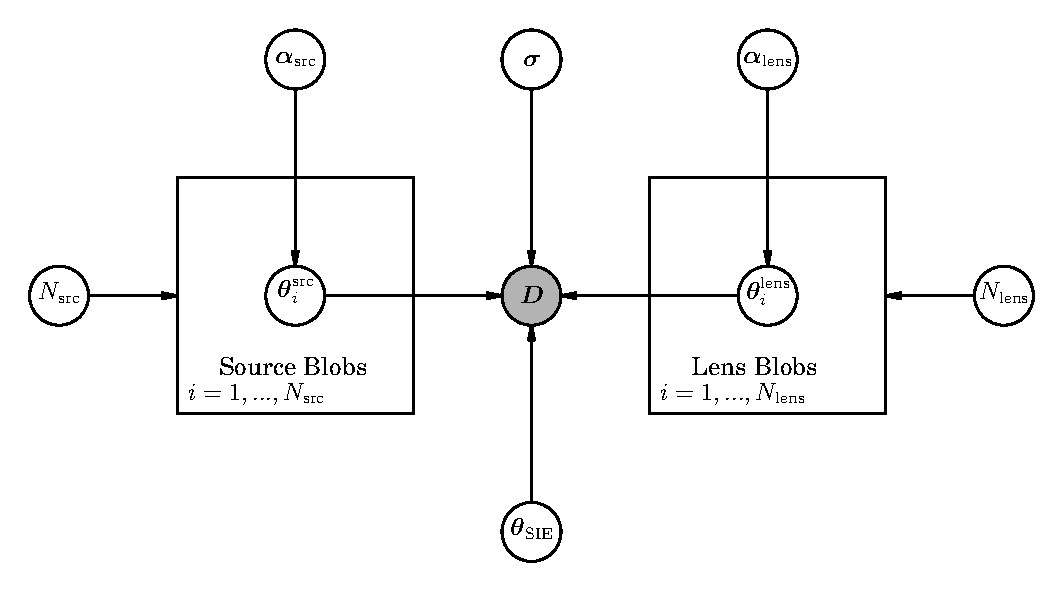
\includegraphics{pgm.pdf}
\caption{A probabilistic graphical model (PGM) of the dependence structure
of the prior information.\label{fig:pgm}}
\end{figure*}


\subsection{The Lens}

The NIE parameters...

A lensing blob with mass $M$ and width $v$
centered at the origin has the following surface mass density profile:
\begin{eqnarray}
\rho(x, y) &=& \left\{
\begin{array}{lr}
\frac{M}{2\pi v^2}\left[1 - \left(\frac{r}{v}\right)^2\right], & r \leq v\\
0, & \textnormal{otherwise}
\end{array}
\right.
\end{eqnarray}
The deflection angles are:


\section{The Cosmic Horseshoe}
As a demonstration the method is the applied to the Cosmic Horseshoe INT data. 
The field of view of the image is $15.3180" \times 15.3180"$, and the size is $46 \times 46$ pixels, therefore one pixel is equivalent to $0.33"$. \\
The method discussed  in the previous section is applied to two models, the first model consist of a flexible source and a Singular Isothermal Elliptical(SIE) model for the lens.  This model is similar to models used in previous work \cite{Belokurov2007} \cite{Dye2008}. 
The second model has in addition to the flexible source and SIE, also possible satellites. \\
The amount of added satellites is automatically determined by the program. If models the addition of an satellite galaxies gives a higher probability it will be preferred over then model without satellite galaxies.  \\
In both models the SIE is specified by the usual parameters: the location of the NIE ($x_c$,$y_c$), b, axis ratio $f$\footnote{in the code denoted with $q$},  the core radius$\zeta$, $\theta$, shear $\gamma$, and $\theta_{\gamma}$ \cite{kormann_schneider_1994}.\\
One of the firsts step in applying Bayesian analysis is providing good prior distribution for the parameters. 
The chosen prior probability distributions are displayed in table \ref{table:1}. The parameters which are not listed in table 
\ref{table:1} depend on parameters which are listed. 

\begin{table}
\centering
\begin{tabular}{ l l}
parameter    &  expression        \\  
\hline 
b            &  $exp\left(  log_{10}(10^{-3})+  log_{10}(10^{3})\cdot Unif(0,1) \right)\cdot scale  $ \\
q            &  $0.05 + 0.95\cdot Unif(0,1) $ \\
$x_c$       &  $0.5\cdot (x_{max} + x_{min}) +   0.1 \cdot(x_{max} - x_{min}) \cdot tan(\pi\cdot ( Unif(0,1) - 0.5)  )$ \\
$		y_c$  &  $0.5\cdot (y_{max} + y_{min}) + 0.1\cdot (y_{max} - y_{min}) \cdot tan(\pi\cdot (Unif(0,1)  - 0.5)  ) $\\
%rc           &  if $\left\{
%  \begin{array}{l l}
%    \textrm{singular} & \quad bb\\
 %   \textrm{non-singular} & \quad  bb
  %\end{array} \right.$
rc(singular)   & $10^{-7}\cdot scale$ \\
rc(non-singular)   & $  exp\left(log_{10}(10^{-3})+  log_{10}(10^{3})\cdot Unif(0,1)\right) \cdot scale   $\\
$\theta$   & $\pi \cdot Unif(0,1)$\\
shear      & $0.05 \cdot tan(\pi \cdot 0.5 \cdot Unif(0,1)) $\\
$theta_{shear}$  & $ \pi\cdot Unif(0,1)$ \\
\end{tabular}
\parbox{0.75\linewidth}{\caption{Prior probabilities distribution for NIE parameters, where the scale parameter depends on <something> \label{table:1} }}

\end{table}


 \begin{figure}[!h]
 \hspace{20pt}
\begin{subfigure}{.45\textwidth}
  \centering
  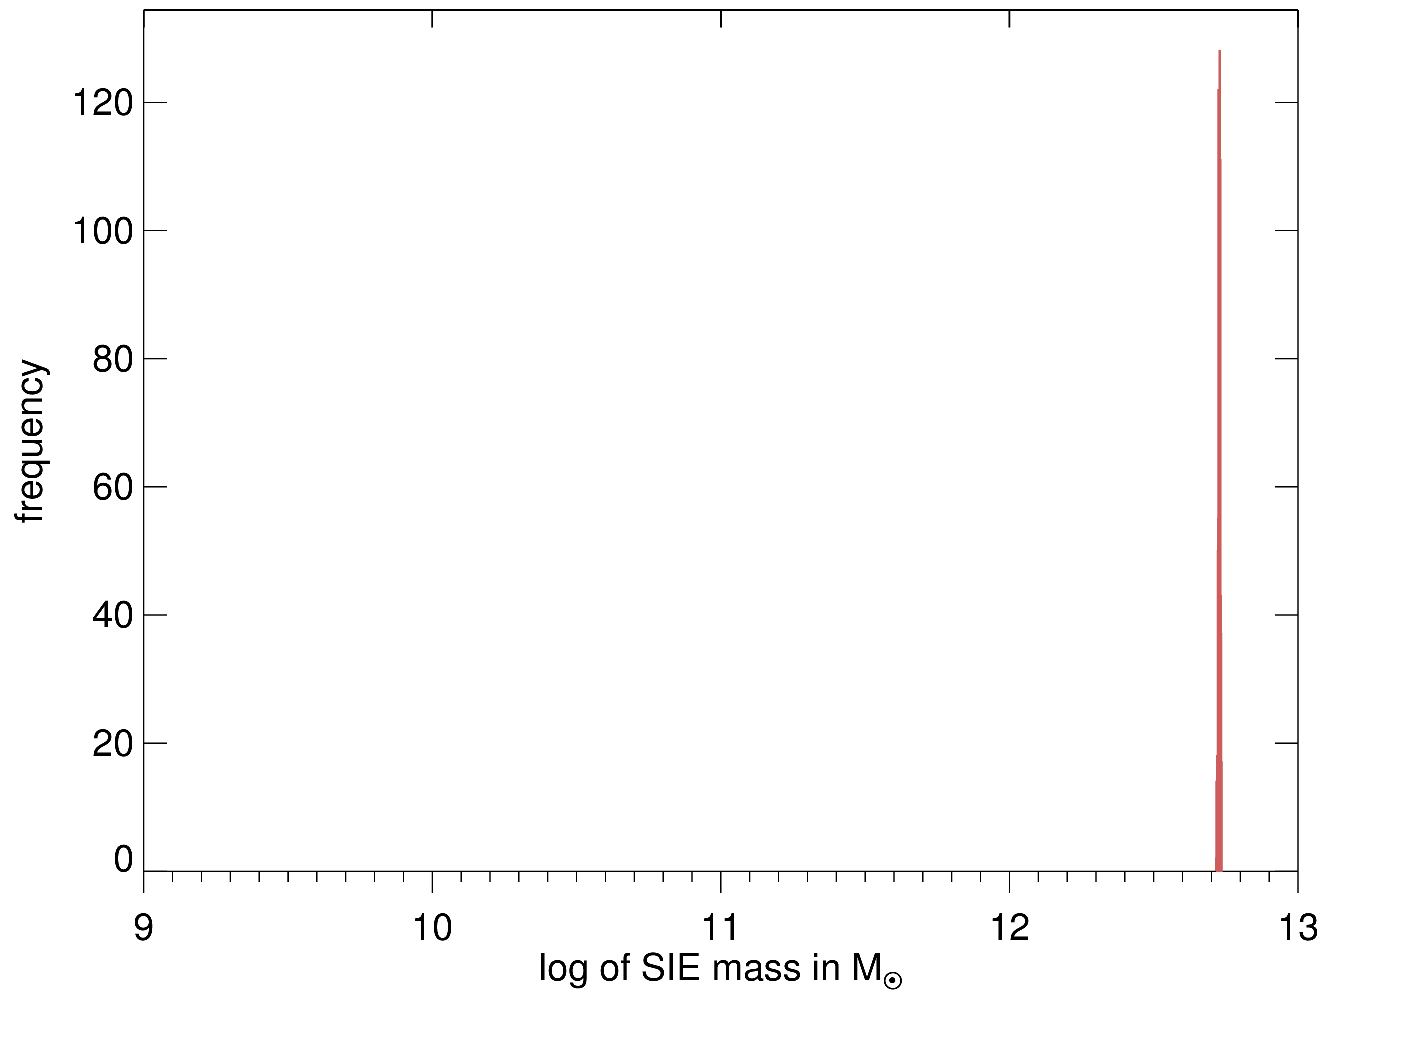
\includegraphics[width=0.75\linewidth,angle=90]{log_mass_SIE_no_blobs.eps}
\parbox{0.8\linewidth}{\caption{The log of the SIE mass within the critical curve  for model A.  \label{fig:sub1} }}
\end{subfigure}%
\begin{subfigure}{.45\textwidth}
  \centering
  
\includegraphics[width=0.75\linewidth,angle=90]{log_mass_SIE.eps}
   \parbox{0.8\linewidth}{\caption{The log of the SIE mass within the critical curve for model B.   \label{fig:sub2}}}
\end{subfigure}
   \end{figure}

After choosing the prior probabilities one has to initialized the Dnest-code, which mean incorporating the problem specific information for
 example dimensions of the images in pixels, image size in arc-seconds, information on the PSF etc in the metadata file. 
 Besides these problem specific parameters, there are also several other parameters concerning the performance of code which need to be
  edited in the OPTION file. After these initialization, we ran a test run to explore the amount of necessary levels, and length of the run.
 A sufficiently amount of levels correlates with good degree of mixing, and the length of the run is associated with the larger sample
  size. After one test run, the amount levels was adapted to 120, and the amount iterations was change to 5000 iterations, for model A this resulted in the effective sample size of 940, and for model B this resulted in the effective sample size of 757.  The difference between the effective sample size is not unexpected, since the probability space which can be explored by applying model B much larger.  \\
Throughout the paper the standard cosmology was used for the analysis:  $H_0=70 \rm{km~s^{-1} ~pc^{-1}}$,  $\Omega_m = 0.3$,and  $\Omega_\Lambda= 0.7$. 
The first test would to compare the SIE-mass of the models with the mass obtained in previous  work \cite{Belokurov2007} \cite{Dye2008}.
Using model A the median  calculated SIE mass within the critical curve in solar masses is  $(5.34 \pm 0.046) \cdot 10^{12} M_\odot$, % (using median + STDDEV)
which is comparable with previous work which gave the enclosed (cylindriacal) mass $(5.4 \pm 0.09) \cdot 10^{12} M_\odot$ \cite{Belokurov2007} and  mass within the Einstein-ring $(5.02 \pm 0.09) \cdot 10^{12} M_\odot$ \cite{Dye2008}. Figure \ref{fig:sub1} displays the histogram of the enclosed mass within an Einstein ring of $5"$, it displays a very well confined probability distribution of the mass. \\ 
Using model B the median calculated SIE mass within the critical curve in solar masses is  $(5.34 \pm 0.046) \cdot 10^{12} M_\odot$, % (using median + STDDEV)
which is slightly smaller compared to the masses obtained with model A and the masses from previous work mentioned above. Which is also not unexpected, because models where the SIE-mass is smaller can compensate by adding a satellite near by. Therefore the distribution is much wider as one can see in figure \ref{fig:sub2}. The median of the SIE-mass in model B is $(4.79 \pm 1.66) \cdot 10^{12} M_\odot$, which leaves a large numerical uncertainty. However by comparison of the two histograms in figure \ref{fig:1} it is apparent that the distribution has a strong feature at the location. \\
 
\begin{figure}[!h]
\hspace{5pt}
\begin{subfigure}{.45\textwidth}
  \centering
  
\includegraphics[width=0.7\linewidth,angle=90]{log_total_mass_blob.eps}
\parbox{0.8\linewidth}{\caption{The log of the total mass of the satellites for model B.   \label{fig:sub3}}}
\end{subfigure}%
\hspace{-15pt}
\begin{subfigure}{.45\textwidth}
  \centering
  \vspace{6pt}
  
\includegraphics[width=0.7\linewidth,angle=90]{log_total_mass_blobs_within_ring.eps}
\parbox{0.8\linewidth}{\caption{The log of the total mass of the satellites within the fixed Einstein-radius for model B.  \label{fig:sub4} }}
\end{subfigure}
   \end{figure}
\vspace{-15pt}
\noindent Another interesting aspect is the mass of the satellites. Figure \ref{fig:sub3} displays a histogram of the logarithm of the total mass of the satellites per sample. Figure \ref{fig:sub4} displays histogram of the logarithm of the total mass of the satellites within a radius of $ 5"$ from the centre of images per sample. Comparing these two images reveals that large part the massive satellites lie outside the Einstein ring. The satellites at a larger distance can only influence the images if they are more massive. Figure \ref{fig:sub5} display a histogram of the log of the total mass of the SIE and the satellites within the Einstein radius, which clearly looks very similar to \ref{fig:sub1}. 
Figure \ref{fig:sub6} display a plot of the total mass of the SIE versus mass of the satellites within the Einstein radius whichs  negative correlation of approximately 
\begin{equation}
 \sum M_{satellites} = 5\cdot10^{12} - M_{SIE}
 \end{equation}

The main conclusion of the analysis of the datasets of model A and model B, would be that the application of the DNest code with a free amount of satellite galaxies return a well matching model which is very similar to to the model without any satellites, this proves 
even though the code has the freedom the explore and create all sort of models, it confirms that the already known distribution is very probable. This shows how well the code works, and beside that it is also good indication that the well established SIE model for this system doesn't need additional satellites to explain the system. 
 
\begin{figure}
\hspace{10pt}
\begin{subfigure}{.5\textwidth}
\vspace{-12pt}
  \centering
  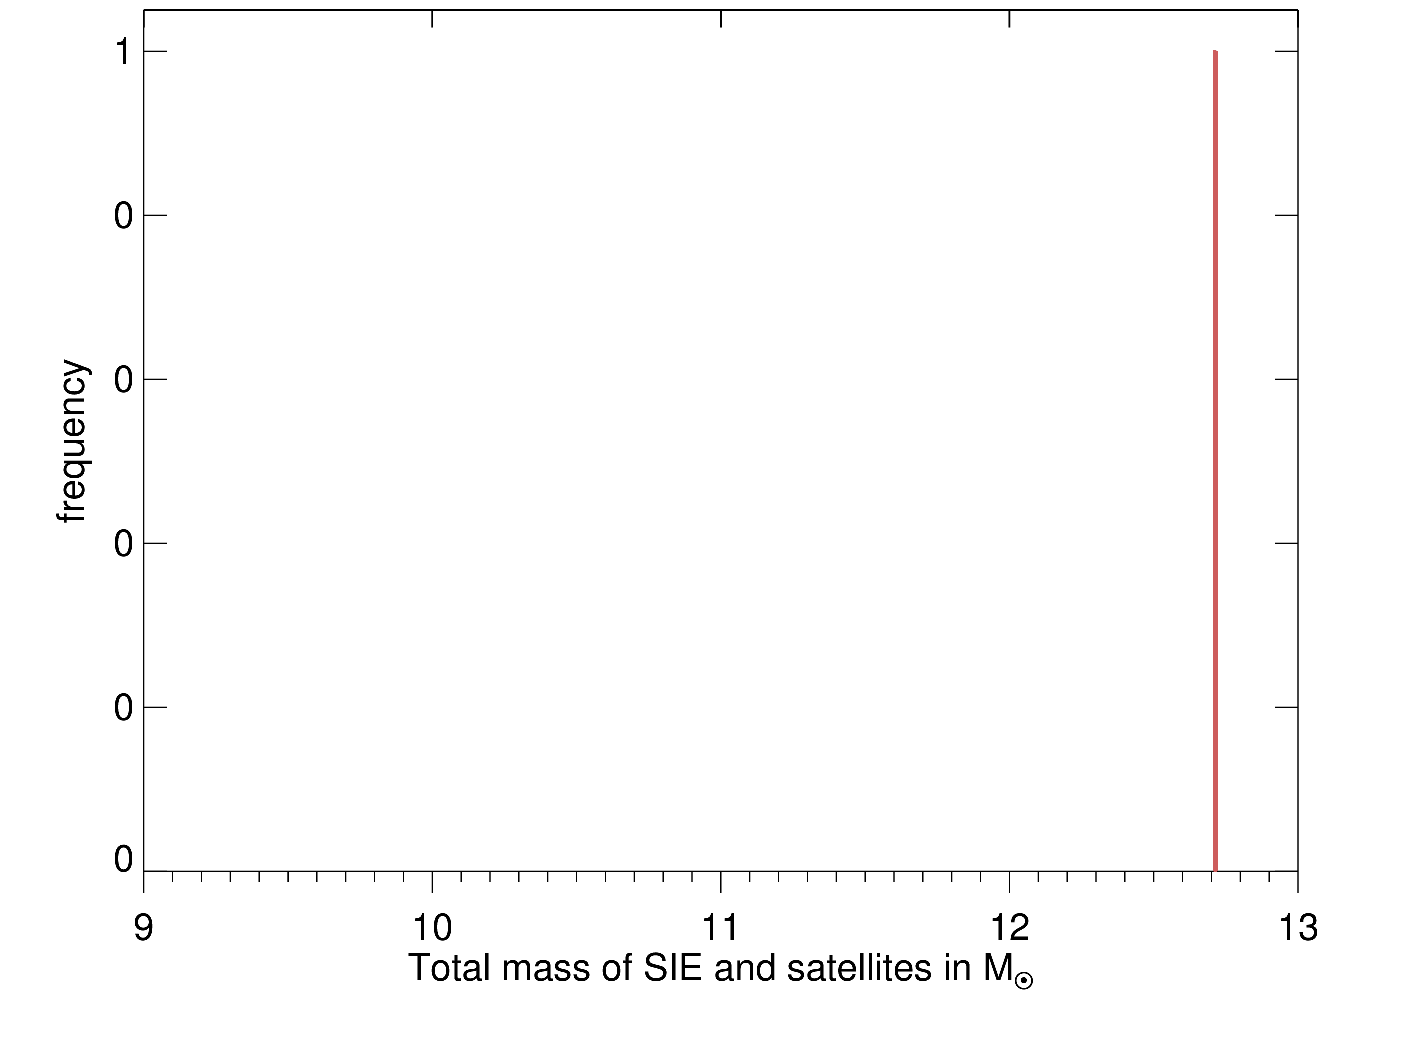
\includegraphics[width=0.75\linewidth,angle=90]{mass_SIE_plus_blob_mass.eps}
\parbox{0.8\linewidth}{\caption{The log of add mass of the satellites and SIE within the fixed Einstein-radius for model B.   \label{fig:sub5}}}
\end{subfigure}
\begin{subfigure}{.5\textwidth}
  \centering
  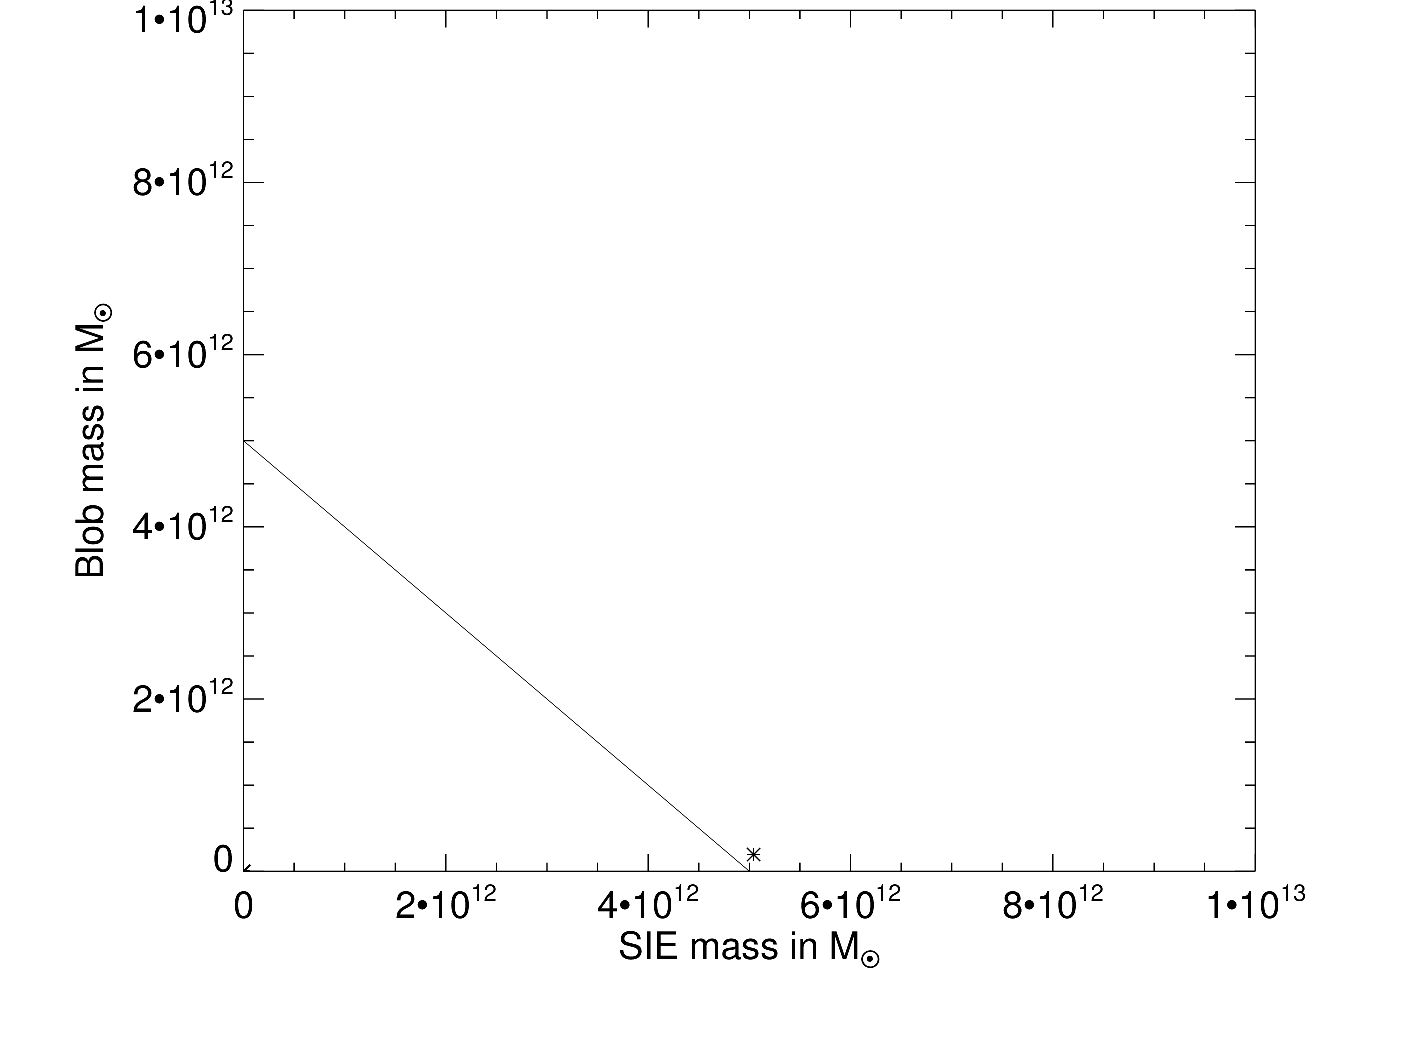
\includegraphics[width=0.75\linewidth,angle=90]{joint.eps}
\parbox{0.8\linewidth}{\caption{Plot of the log of the total mass of the satellites within the fixed Einstein-radius versus the 
log of the SIE mass within the Einstein radius for model B.  \label{fig:sub6} }}
\end{subfigure}

   \end{figure}

  
  

\section{ER 0047-2808}
We demonstrate the method on the HST images of ER 0047-2808.




\begin{thebibliography}{99}
\bibitem[\protect\citeauthoryear{Brewer, P{\'a}rtay,
\& Cs{\'a}nyi}{2011}]{dnest} Brewer B.~J., P{\'a}rtay L.~B., Cs{\'a}nyi G., 2011,
Statistics and Computing, 21, 4, 649-656. arXiv:0912.2380

\bibitem[\protect\citeauthoryear{Brewer et al.}{2011}]{2011MNRAS.412.2521B} 
Brewer B.~J., Lewis G.~F., Belokurov V., Irwin M.~J., Bridges T.~J., Evans 
N.~W., 2011, MNRAS, 412, 2521

\bibitem[\protect\citeauthoryear{Brewer}{2014}]{rjobject} Brewer, B. J., 2014,
preprint. ArXiv: 1411.3921

\bibitem[\protect\citeauthoryear{Coles, Read, 
\& Saha}{2014}]{2014MNRAS.445.2181C} Coles J.~P., Read J.~I., Saha P., 2014, MNRAS, 445, 2181

\bibitem[\protect\citeauthoryear{O'Hagan and Forster}{2004}]{ohagan}
O'Hagan, A., Forster,~J., 2004, Bayesian inference. London: Arnold.

\bibitem[\protect\citeauthoryear{Sivia \& Skilling}{2006}]{sivia} Sivia, 
D.~ S., Skilling, J., 2006, Data Analysis: A Bayesian Tutorial, 2nd 
Edition, Oxford University Press

\bibitem[\protect\citeauthoryear{Skilling}{2006}]{skilling} Skilling, 
J., 2006, ``Nested Sampling for General Bayesian Computation'', Bayesian 
Analysis 4, pp. 833-860

\bibitem[\protect\citeauthoryear{Suyu et al.}{2006}]{suyu} 
Suyu S.~H., Marshall P.~J., Hobson M.~P., Blandford R.~D., 2006, MNRAS, 
371, 983

\bibitem[\protect\citeauthoryear{Treu}{2010}]{treu} Treu T., 2010, ARA\&A, 48, 87 

\bibitem[\protect\citeauthoryear{Vegetti et 
al.}{2012}]{vegetti1} Vegetti S., Lagattuta D.~J., McKean J.~P., 
Auger M.~W., Fassnacht C.~D., Koopmans L.~V.~E., 2012, Natur, 481, 341 

\bibitem[\protect\citeauthoryear{Vegetti et 
al.}{2010}]{vegetti2} Vegetti S., Koopmans L.~V.~E., Bolton A., 
Treu T., Gavazzi R., 2010, MNRAS, 408, 1969 

\bibitem[\protect\citeauthoryear{Vegetti, Czoske, 
\& Koopmans}{2010}]{vegetti3} Vegetti S., Czoske O., Koopmans L.~V.~E., 2010, MNRAS, 407, 225

\bibitem[\protect\citeauthoryear{Warren 
\& Dye}{2003}]{2003ApJ...590..673W} Warren S.~J., Dye S., 2003, ApJ, 590, 673
\end{thebibliography}


\end{document}

